\documentclass[12pt,a4paper]{article}
\usepackage{geometry}
\geometry{left=2.5cm,right=2.5cm,top=2.0cm,bottom=2.5cm}
\usepackage[english]{babel}
\usepackage{amsmath,amsthm}
\usepackage{amsfonts}
\usepackage[longend,ruled,linesnumbered]{algorithm2e}
\usepackage{fancyhdr}
\usepackage{ctex}
\usepackage{array}
\usepackage{listings}
\usepackage{color}
\usepackage{graphicx}
\usepackage{url}
\usepackage{hyperref}
\hypersetup{hidelinks}
\usepackage{longtable}
\usepackage{booktabs}
\usepackage{amsmath}
\usepackage{listings}

\lstset{
    basicstyle=\ttfamily\small,
    frame=single,
    breaklines=true,
    postbreak=\mbox{\textcolor{red}{$\hookrightarrow$}\space},
    showstringspaces=false,
    commentstyle=\color{gray},
    keywordstyle=\color{blue}
}

\begin{document}

\title{智能计算体系结构Lab2实验报告}
\date{}

\author{
姓名:\textbf{卞卓航}~~~~~~
学号:\textbf{22373017}~~~~~~
}

\maketitle

\section{实验说明}

由于本次实验框架提供的代码为\texttt{tensorflow1.15}版本,所支持的最高CUDA版本为\texttt{CUDA10.0},而我的电脑上的CUDA版本为\texttt{CUDA11.8}。

相较于折腾CUDA和重写实验代码,显然使用·\texttt{tensorflow2.x}版本重写一遍实验是一种更为方便的方法,并且不会有折腾坏CUDA的风险。

本次实验最终\textbf{没有采用提供的模板代码},而是使用了\texttt{tensorflow2.13}版本进行书写。

\section{实验目标}

本次实验的目标为搭建深度神经网络,实现一个\texttt{LeNet},来完成在\texttt{MINIST}数据集上的数字识别任务。

相较于\texttt{1.x}版本,\texttt{2.x}版本的\texttt{tensorflow}提供了较好层次的抽象,使得在代码书写上较为简易。

\section{实验原理}

\subsection{CNN:卷积神经网络}

卷积神经网络依旧是层级网络,只是层的功能和形式做了变化,可能会多原有层级网络没有的部分。

\subsubsection{层级结构}

一个卷积神经网络主要由以下5层组成:

\begin{itemize}
\item
  数据输入层:Input layer
  
  该层要做的处理主要是对原始图像数据进行预处理,其中包括:
    \begin{itemize}
    \item
      去均值:把输入数据各个维度都中心化为0,其目的就是把样本的中心拉回到坐标系原点上。
    \item
      归一化:幅度归一化到同样的范围,即减少\textbf{各维度数据取值范围的差异}而带来的干扰
    \item
      PCA/白化:用PCA降维;白化是对数据\textbf{各个特征轴上的幅度归一化}
    \end{itemize}
\item
  卷积计算层:CONV layer

  在这个卷积层,有两个关键操作:

    \begin{itemize}
    \item
      局部关联。每个神经元看做一个滤波器(filter)
    \item
      窗口(receptive field)滑动, filter对局部数据计算
    \end{itemize}
\item
  ReLU激励层:ReLU layer
\item
  池化层:Pooling layer
\item
  全连接层:FC layer
\end{itemize}

\subsubsection{相关名词}

\begin{itemize}
\item
  深度depth:数据的层数
\item
  步幅stride:窗口一次滑动的长度
\item
  填充值zero-padding
\end{itemize}

\subsection{LeNet}

Lenet是一系列网络的合称,包括Lenet1-Lenet5,是卷积神经网络的开山之作,也是将深度学习推向繁荣的一座里程碑。

LeNet首次采用了卷积层、池化层这两个全新的神经网络组件,接收灰度图像,并输出其中包含的手写数字,在手写字符识别任务上取得了瞩目的准确率。LeNet网络的一系列的版本,以LeNet-5版本最为著名,也是LeNet系列中效果最佳的版本。

\section{实验实现}

参照提供的模板代码,以类似的文件逻辑结构书写了相关的网络代码。

\subsection{网络定义}

在\texttt{tf\_network.py}中实现了对网络的定义

\begin{lstlisting}
# 计算输入层
self.net = keras.Sequential([
    # layer1
    Conv2D(self.filters, kernel_size=self.kernel_size),
    MaxPooling2D(pool_size=2, strides=2),
    ReLU(),

    # layer2
    Conv2D(16, kernel_size=self.kernel_size),
    MaxPooling2D(pool_size=2, strides=2),
    ReLU(),

    # layer3
    Conv2D(120, kernel_size=self.kernel_size),
    ReLU(),
    Flatten(),

    # fc1
    Dense(84, activation='relu'),

    # fc2
    Dense(10, activation='softmax')
])
\end{lstlisting}

\subsection{不同层的定义}

\begin{itemize}
\item
  \textbf{layer1}:

  \begin{itemize}
  \item
    \texttt{Conv2D(self.filters,\ kernel\_size=self.kernel\_size)}:二维卷积层,用于提取输入数据的特征。

    \begin{itemize}
    \item
      \texttt{self.filters} 指定了卷积核的数量
    \item
      \texttt{kernel\_size=self.kernel\_size} 指定了卷积核的大小
    \end{itemize}
  \item
    \texttt{MaxPooling2D(pool\_size=2,\ strides=2)}:最大池化层,用于降低特征图的空间维度(高和宽),同时保留最重要的信息

    \begin{itemize}
    \item
      \texttt{pool\_size=2} 表示池化窗口的大小为 2x2
    \item
      \texttt{strides=2} 表示池化窗口移动的步长为 2
    \end{itemize}
  \item
    \texttt{ReLU()}:这是一个激活层,使用 ReLU(Rectified Linear
    Unit)激活函数来引入非线性

    \begin{itemize}
    \item
      ReLU 函数的公式是 \texttt{f(x)\ =\ max(0,\ x)}
    \end{itemize}
  \end{itemize}
\item
  \textbf{layer2}:

  \begin{itemize}
  \item
    \texttt{Conv2D(16,\ kernel\_size=self.kernel\_size)}:二维卷积层

    \begin{itemize}
    \item
      这次卷积核的数量是16
    \item
      经过这一层,6 张\texttt{14\ x\ 14}的feature
      map变成了16张\texttt{14\ x\ 14}的feature map
    \end{itemize}
  \item
    \texttt{MaxPooling2D(pool\_size=2,\ strides=2)}:最大池化层,与
    layer1 中的相同
  \item
    \texttt{ReLU()}:另一个 ReLU 激活层
  \end{itemize}
\item
  \textbf{layer3}:

  \begin{itemize}
  \item
    \texttt{Conv2D(120,\ kernel\_size=self.kernel\_size)}:第三个二维卷积层,卷积核的数量是
    120
  \item
    \texttt{ReLU()}:这是第三个 ReLU 激活层
  \item
    \texttt{Flatten()}:这是一个展平层,用于将多维的特征图转换为一维向量

    \begin{itemize}
    \item
      这对于将卷积层的输出传递给全连接层是必要的。
    \end{itemize}
  \end{itemize}
\item
  \textbf{fc1}:

  \begin{itemize}
  \item
    \texttt{Dense(84,\ activation=\textquotesingle{}relu\textquotesingle{})}:全连接层

    \begin{itemize}
    \item
      有 84 个神经元,使用 ReLU 激活函数。
    \end{itemize}
  \end{itemize}
\item
  \textbf{fc2}:

  \begin{itemize}
  \item
    \texttt{Dense(10,\ activation=\textquotesingle{}softmax\textquotesingle{})}:全连接层

    \begin{itemize}
    \item
      使用 \texttt{softmax} 激活函数可以将输出转换为概率分布
    \end{itemize}
  \end{itemize}
\end{itemize}

\subsection{数据来源}

使用了\texttt{tensorflow}中内置的MINST数据集,在\texttt{tf\_data.py}中实现了对数据的解析。

\subsubsection{数据填充}

使用填充函数对图像进行了填充,将尺寸由\texttt{28*28}填充为了\texttt{32*32},在不足处填补0。

\begin{lstlisting}
# padding 28*28 to 32*32
paddings = tf.constant([[0, 0], [2, 2], [2, 2]])
x_train = tf.pad(x_train, paddings)
x_test = tf.pad(x_test, paddings)
\end{lstlisting}

\subsubsection{独热码转换}

\begin{enumerate}
\def\labelenumi{\arabic{enumi}.}
\item
  将输入的特征数据转换为浮点型,并将其值归一化到0到1之间:原始的MNIST数据集中的图像像素值范围是0到255,归一化可以帮助模型更好地学习
\item
  将特征数据重塑为\texttt{{[}-1,\ 32,\ 32,\ 1{]}}的形状,其中\texttt{-1}表示自动计算该维度的大小,以确保数据的总元素数量不变
\item
  对标签数据进行one-hot编码。将整数类型的标签转换为长度为10的向量,其中只有一个元素为1,其余元素为0。目的是为了让模型能够处理分类问题
\end{enumerate}

\begin{lstlisting}
def _dense_to_one_hot(x, y):
    x = tf.cast(x, dtype=tf.float32) / 255.
    x = tf.reshape(x, [-1, 32, 32, 1])
    y = tf.one_hot(y, depth=10)  # one_hot 编码
    return x, y
\end{lstlisting}

\subsection{训练流程}

对网络的建立、训练、测试保存均进行了封装,直接运行\texttt{tf\_minst.py}文件即可。

\begin{lstlisting}
train_db, test_db = get_train_test_data()

net = LeNet(input_shape=(batch_size, 32, 32, 1))
net.summary()

# train
history = net.train(train_db,
                    epoch=epoch,
                    lr=lr,
                    batch_size=batch_size,
                    log_dir=log_dir)
# test
net.test(test_db)

# save
net.save()
\end{lstlisting}

\section{实验结果与分析}

\subsection{默认实验配置}

对于基本的参数设置(\texttt{lr=0.01}),测试准确率为0.88

准确率变化:

\begin{figure}[htbp]
    \centering
    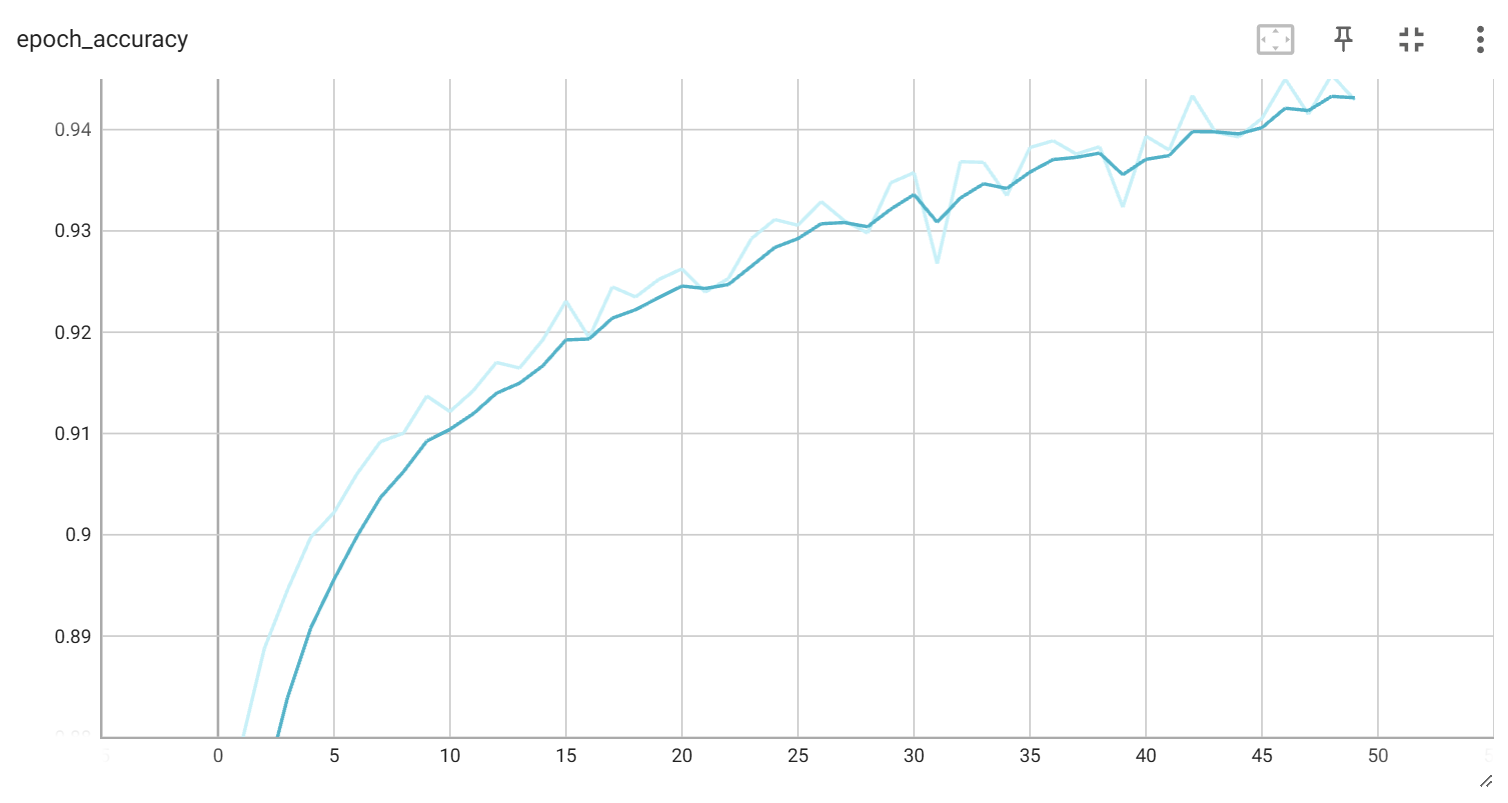
\includegraphics[width=0.6\linewidth]{img/accuracy_graph.png}
    \caption{accuracy graph}
\end{figure} 

loss变化:

\begin{figure}[htbp]
    \centering
    \includegraphics[width=0.6\linewidth]{img/loss_grapg.png}
    \caption{loss grapg}
\end{figure} 

\subsection{调参分析}

分别改变了学习率和最后一层的激活函数。

\subsubsection{学习率lr}

对于不同学习率,记录了参数:

\begin{table}[htbp]
    \centering
    \caption{不同学习率的准确率比较}
    \begin{tabular}{ll}
        \toprule
        学习率 & 准确率 \\
        \midrule
        0.01 & 0.88670 \\
        0.02 & 0.88584 \\
        0.03 & 0.84134 \\
        0.04 & 0.10029 \\
        0.05 & 0.09327 \\
        \bottomrule
    \end{tabular}
\end{table}

并且注意到,在训练过程中也会出现类似的波动:

\begin{figure}[htbp]
    \centering
    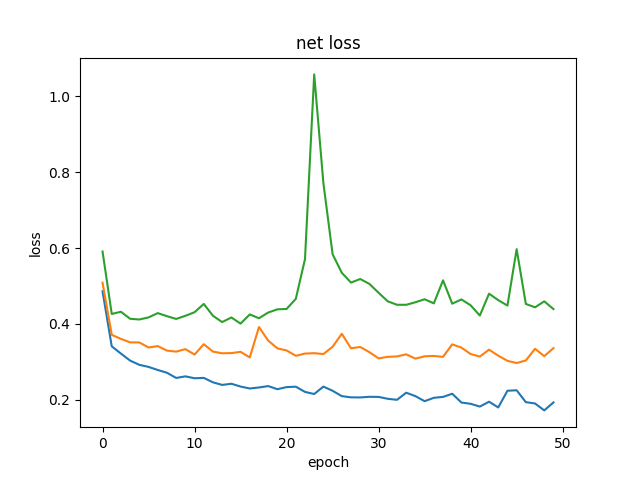
\includegraphics[width=0.5\linewidth]{img/loss_wave.png}
    \caption{loss wave}
\end{figure} 

在lr增大时尤为明显:

\begin{figure}[htbp]
    \centering
    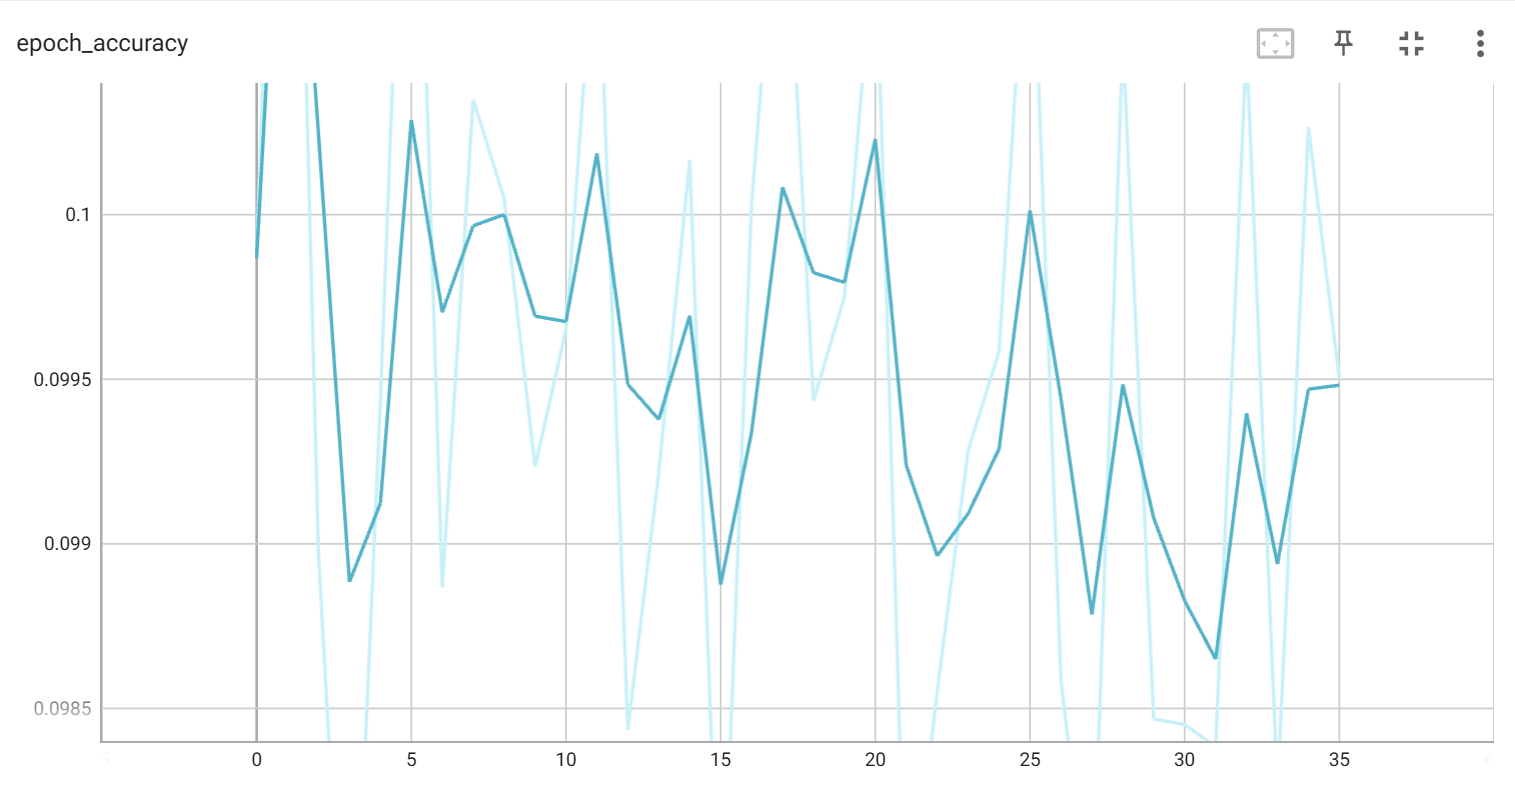
\includegraphics[width=0.6\linewidth]{img/accuracy_wave.png}
    \caption{accuracy wave}
\end{figure} 

\subsubsection{激活函数}

对于不同的激活函数,有:

\begin{table}[htbp]
    \centering
    \caption{不同激活函数的准确率比较}
    \begin{tabular}{ll}
        \toprule
        激活函数 & 准确率 \\
        \midrule
        softmax & 0.88670 \\
        sigmoid & 0.88200 \\
        relu & 0.10000 \\
        tanh & 0.10000 \\
        \bottomrule
    \end{tabular}
\end{table}

\section{实验总结}

使用\texttt{tensorflow}完成了一个\texttt{LeNet},对于深度学习框架有了一定的了解,巩固了对CNN的认识。

\end{document}